\section{Conventions de représentations}

\subsection{Présentation de la convention retenue}
L'algorithme prend un graphe dirigé en entrée et retourne un booléen, qui indique si le graphe possède un cycle ou non. Il nous faut donc définir une convention de représentation d'un graphe dirigé sur lequel notre algorithme va s'appliquer. \\

Le graphe sera représenté en utilisant la matrice d'adjacence. Cette matrice est une matrice carrée dont la dimension est égale au nombre de noeuds du graphe. Chaque entrée $(i,j)$ avec $0\leq i,j \leq n-1$ indique le nombre d'arêtes allant du noeud $i$ au noeud $j$.\\

Nous donnons ici un exemple d'une telle représentation. Le graphe donné ci-dessous sera représenté par le tableau suivant :
\begin{multicols}{2}
\begin{center}
\begin{tabular}{c|ccccc}
&0 & 1 & 2 & 3 & 4\\
\hline
0&0&1&0&0&0\\
1&0&0&1&0&0\\
2&1&0&0&0&0\\
3&0&1&0&0&0\\
4&0&0&0&1&0\\
\end{tabular}
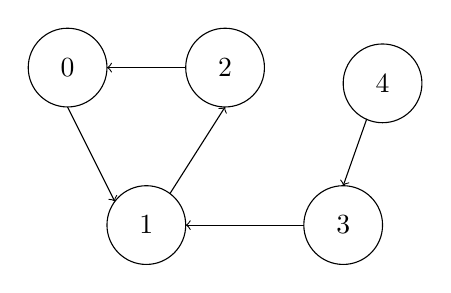
\begin{tikzpicture}
\draw (1,0) circle (0.5) ;
\draw (1,0) node {1} ;
\draw[->] (1.3,0.4) -- (2,1.5);
\draw (2,2) circle (0.5);
\draw (2,2) node {2} ;
\draw[->] (1.5,2) -- (0.5,2);
\draw (0,2) circle (0.5);
\draw (0,2) node {0} ;
\draw[->] (0,1.5) -- (0.6,0.3);
\draw (3.5,0) circle (0.5);
\draw (3.5,0) node {3} ;
\draw[->] (3,0) -- (1.5,0);
\draw (4,1.8) circle (0.5);
\draw (4,1.8) node {4} ;
\draw[->] (3.8,1.35) -- (3.5,0.5);
\end{tikzpicture}
\end{center}
\end{multicols}

\subsection{Motivations}
Le fait de représenter un graphe par le tableau à double entrée décrit précédemment possède divers avantages. Ceux-ci sont les suivants : \\

\begin{itemize}
\item \textbf{Facilité d'implémentation} : dans l'algorithme à implémenter, les actions principales à effectuer sur le graphe sont de parcourir les noeuds, de déterminer si ils ont des arêtes entrantes et de les supprimer. L'implémentation de ces deux fonctionnalités devient très facile. En effet, pour le parcours des noeuds, il suffit de parcourir le tableau à l'aide de boucles sur ses indices. Pour déterminer si un noeud $j$ n'a aucune arête entrante, il suffit que la somme des éléments de la $j$ème colonne de la matrice d'adjacence soit nulle. Pour la suppression, il suffit de marquer la ligne et la colonne associées au noeud comme ne devant plus être parcourues.

\item \textbf{Complexité satisfaisante} : on déduit de ce qui a été dit au point précédent que la recherche d'un noeud sans arrêtes entrantes se fait en $O(n^2)$ et que la suppression de celui-ci (ou plus précisément le marquage dans notre cas) se fait en $O(1)$. Ces complexités étant polynomiales, celles-ci sont considérées comme efficaces. De plus, d'autres représentations possibles ont été considérées et aucune ne donnait une meilleure complexité pour la recherche et la suppression.

\item \textbf{Marquage} : il a été décidé de marquer la ligne et la colonne associées à un noeud à supprimer au lieu de les supprimer du tableau. En effet, cela évite de devoir recopier le tableau dans un tableau de plus petite taille, ce qui est une opération qui se fait en $O(n^2)$ alors que le marquage se fait en $O(1)$.
\end{itemize}
